\chap{Astuces pour utiliser les \emph{sliders}}\label{a.tech}

\sect{Régler les \emph{sliders} dans les blocs moteurs}

Il est difficile de régler précisément les \emph{sliders}, par exemple pour que les deux
moteurs tournent à la même vitesse.
Pour améliorer la précision, nous pouvons utiliser la traduction des paires événement-actions
dans le programme textuel AESL.

\trickbox{Vous remarquerez que déplacer les \emph{sliders} des blocs action moteurs
change la vitesse cible des moteurs (\p{motor.X.target}) par palliers de 50,
entre $-$500 et 500.
En déplaçant délicatement ces \emph{sliders}, vous pouvez choisir toutes ces valeurs comme vitesses.}

La \cref{fig.textcode} montre le programme de la \cref{fig.likes-hates} (celle où votre animal
de companie vous aime et vous suit partout) ainsi que la traduction textuelle, visible sur la droite
de la fenêtre VPL.
Ce texte change automatiquement quand vous déplacez les \emph{sliders}.

\begin{figure}[hbt]
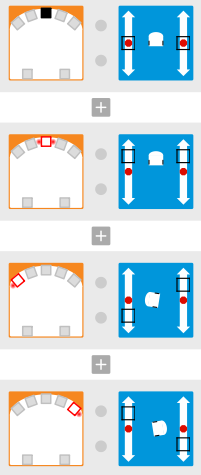
\includegraphics[width=0.3\textwidth]{likes}
\hfill
\begin{minipage}[b]{0.55\textwidth}
\begin{footnotesize}
\begin{verbatim}
onevent prox
    if prox.horizontal[2] < 1000 then
        motor.left.target = 0
        motor.right.target = 0
    end
    if prox.horizontal[2] > 2000 then
        motor.left.target = 300
        motor.right.target = 300
    end
    if prox.horizontal[0] > 2000 then
        motor.left.target = -300
        motor.right.target = 300
    end
    if prox.horizontal[4] > 2000 then
        motor.left.target = 300
        motor.right.target = -300
    end
\end{verbatim}
\end{footnotesize}
\vspace*{8ex}
\end{minipage}
\caption{Un programme VPL et le programme textuel correspondant.}
\label{fig.textcode}
\end{figure}

\p{onevent prox} signifie: chaque fois que l'événement de l'échantillonage des capteurs horizontaux
(les capteurs de \emph{proximité}, ici abbregé \emph{prox}) est déclanché,
les instructions jusqu'au \p{end} suivant seront exécutées.
L'événement proximité se produit 10 fois par seconde.

Lorsqu'un événement se produit, les valeurs des capteurs sont verifiées grâce aux strucutres de condition.
Le capteur numéro 2 (avant central) est verifié en premier: \p{prox.horizontal[2]}.
Si cette valeur est inférieure à 1000, les vitesses des moteurs gauches et droits sont mises à 0
grâce aux instructions:

\begin{footnotesize}
\begin{verbatim}
motor.left.target = 0
motor.right.target = 0
\end{verbatim}
\end{footnotesize}

Chaque structure \p{if ... then ... end} vérifie un capteur spécifique et exécute les instructions
associées si le résultat du test est vrai.
Le programme exécute en fait l'algorithme suivant:

\begin{enumerate}[start=0,noitemsep,nosep]
\item Vérifie que rien ne soit en face; si c'est le cas, le robot s'arrête.
\item Vérifie si quelque chose est en face; si c'est le cas, le robot avance.
\item Vérifie s'il y a quelque chose à gauche; si oui, tourne à gauche.
\item Vérifie s'il y a quelque chose à droite; si oui, tourne à droite.
\end{enumerate}

Une fois que les valeurs de tous les capteurs ont été lues et que l'action appropriée a été exécutée,
le programme attend le prochain événement \p{prox} et recommence les tests.
Ceci se répéte tant que le programme n'est pas arrêté.

\sect{Régler la durée du minuteur}

\trickbox{La durée du bloc action minuteur peut être réglé par multiples de quarts de seconde
(250 millisecondes) jusqu'à quatre secondes.}


\sect{Le bloc événement capteurs en mode avancé}

Cette section décrit les fonctionnalités des blocs événement capteurs disponibles en mode avancé.

\subsection*{Régler les seuils des capteurs}

En mode débutant, les seuils des capteurs sont fixés.
Pour les capteurs horizontaux, une valeur supérieure à 2000 signifie que beaucoup de lumière
est réféchie et un événement sera déclanché si le carré correspondant est blanc,
tandis qu'une valeur inférieure à 1000 signifie que peu de lumière est réfléchie 
et un événement sera déclanché si le carré correspondant est noir.
Pour les capteurs du bas, les seuils sont 450 et 400.

En mode avancé, les seuils peuvent être réglés. Le \emph{slider} du haut permet de régler le seuil
au-dessus duquel un événement blanc se produit et le \emph{slider} du bas permet de régler le seuil
au-dessous duquel un événement noir se produit:\label{p.proximity-sensitivity}

\begin{center}
\begin{tabular}{c@{\hspace{.1\textwidth}}c}
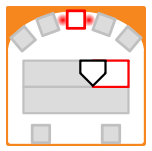
\includegraphics[width=.15\textwidth,keepaspectratio=true]{set-red}
&
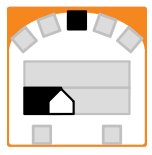
\includegraphics[width=.15\textwidth,keepaspectratio=true]{set-black}
\end{tabular}
\end{center}

La \Cref{fig.follow-line-adv} montre le programme pour suivre une ligne
(\cref{fig.follow-line-all}) en mode avancé.
Les \emph{sliders} ont été réglés de sorte à obtenir des seuils très faibles:
100 à la fois pour le seuil supérieur et inférieur.

\begin{figure}
\subfigure[Démarrer et arrêter le robot]%
{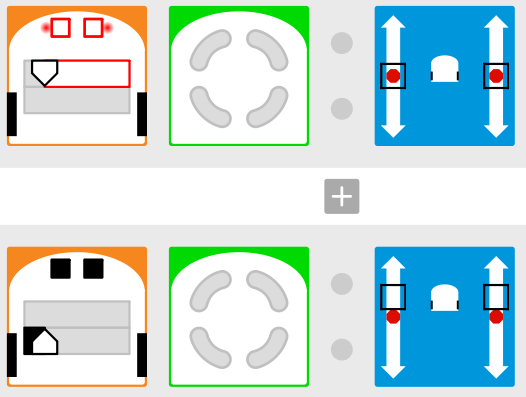
\includegraphics[width=0.45\textwidth]{line-forward-adv}}
\hfill
\subfigure[Corriger quand le robot dévie]%
{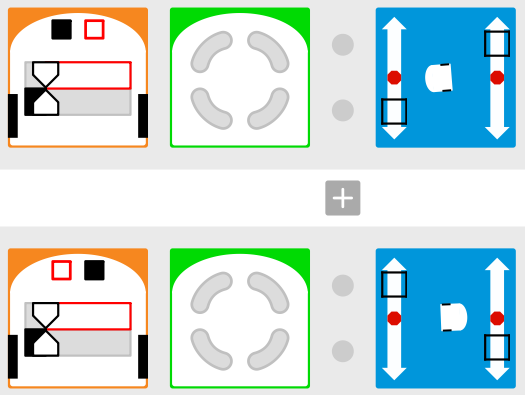
\includegraphics[width=0.45\textwidth]{line-controller-adv}}
\caption{Un programme pour suivre une ligne}
\label{fig.follow-line-adv}
\end{figure}

\subsection*{Plusieurs capteurs}

Si plusieurs capteurs sont activés dans un bloc événement, ils partagent les mêmes seuils:
\begin{center}
\begin{tabular}{c@{\hspace{.1\textwidth}}c}
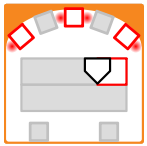
\includegraphics[width=.15\textwidth,keepaspectratio=true]{set-same}
&
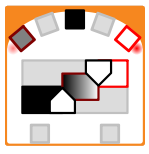
\includegraphics[width=.15\textwidth,keepaspectratio=true]{set-all}
\end{tabular}
\end{center}

\subsection*{Déclancher des événements pour des valeurs entre deux seuils}

Il existe un mode additionnel représenté par un carré gris foncé: \gr{set-gray}{.15}
Dans ce mode, un événement se produit si la valeur mesurée est supérieure au seuil inférieur (réglé
par le \emph{slider} inférieur) et inférieure au seuil supérieur (réglé par le \emph{slider} supérieur).
